\chapter{Topological Persistence and Persistent Homology}
\graphicspath{ {/home/tomasp/Dokumenty/Master_Thesis/figures/} }

The \textit{Niyogi-Smale-Weinberger} theorem tells us that it is possible to hope to recover the underlying topology and structure of the space from a limited number of samples from some experiment or study when the distance between the samples is smaller than what is referred to as its \textit{feature scale}.

The problem now lies in finding this feature scale of the object, since this is usually unknowable in advance outside of simulations. Simultaneously, limiting ourselves to looking for a single value of $\varepsilon$ is not the right path either. Some features of the object may become visible for different values of $\varepsilon$, i.e., regions may connect at smaller distances and holes may be created at larger ones. Neither of the two is intrinsically more valuable than the other without additional context. As such, this should motivate us to instead look at multiple feature scales at once and observe the changes in the homology groups for a range of values of $\varepsilon$. Features that exist for a wider range of values are more likely to be more informative about the underlying structure than features that only live for short intervals.

\begin{figure}[h!]
  \centering
  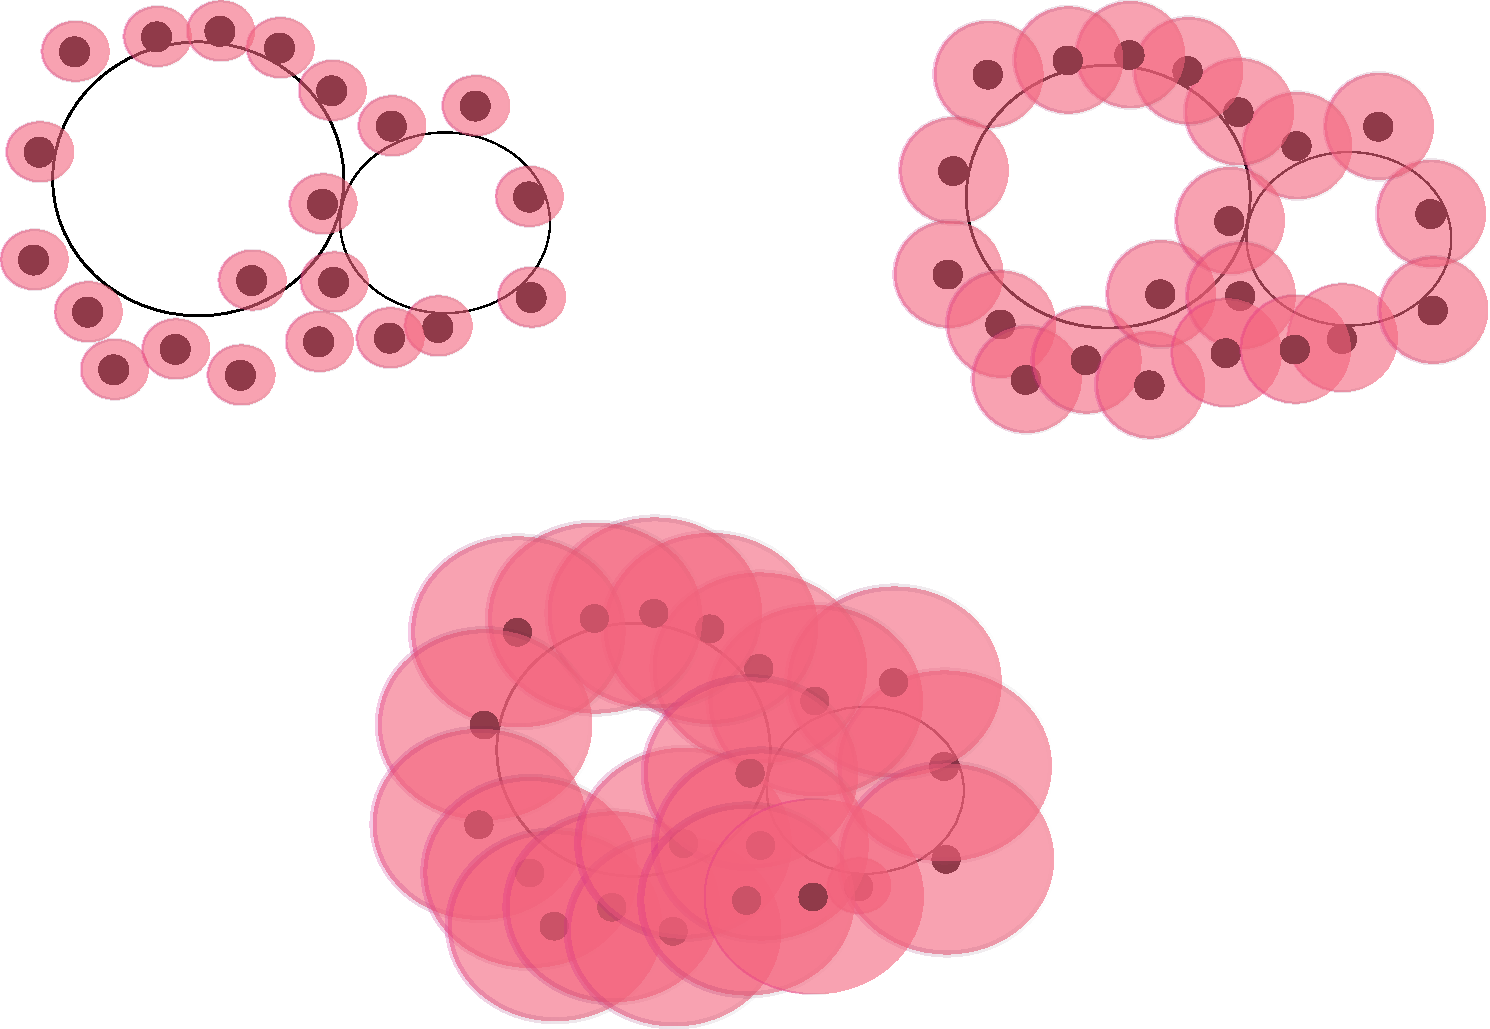
\includegraphics[width=9cm, height=6cm]{filtration_01.pdf}
  \caption{A random sample of points from two touching circles and the growing sublevel sets of the distance function to the points.}
  \label{fig:filtration_01}
\end{figure}

We can consider the point cloud $P$ in \ref{fig:filtration_01} sampled from a curve. Ideally, the goal would be to confirm the existence of one connected component, the two circles touching together, and the presence of two holes, i.e., two loops in total. Even better, we would like to see that one loop is larger and more prominent than the other. This is what the main tool of our work captures -- \textit{persistent homology}.

If we consider the distance function $r: \mathbb{R}^{2} \to \mathbb{R}$, where $r(x) = d(x, P)$, the minimum distance of $x$ to the points in $P$. Taking a look at the sublevel sets of $r$, $r^{-1}[-\infty, a]$ for some $a \in \mathbb{R}^{+} \cup \{0\}$. In this instance, the sublevel sets are unions of closed balls of radius $a$ with the center being the points. By increasing the $a$ from $0$ to infinity, numerous holes will appear, but only the two large loops will live longer than the rest until the entirety of $P$ is covered.

The idea is to translate this rate of survival on the level of points to the survival of individual homology classes whenever we increase the sublevel sets. This is robust since topological ``noise'' dies out quickly in comparison to the interesting topological features. Persistent homology effectively takes a function defined on the topological space and observes the evolution of homology classes over increasing sublevel sets of the function.

It should be noted that there are two different scenarios where persistence takes place. One is where our function is defined on a topological space, which would require the use of singular homology; previously established to be computationally intractable. The other, the one we are interested in, is the case where the function is defined on a simplicial complex. The sequence of sublevel sets there is simply the nested sequence of subcomplexes, usually referred to as a \textit{filtration}. Naturally, here we will be working with simplicial homology, which we know how to efficiently compute.

\subsection{Filtration and persistence}
\subsubsection{Space filtration of topological spaces}

Let $f: \mathbb{T} \to \mathbb{R}$ be a function defined on a topological space $\mathbb{T}$. If we denote $\mathbb{T}_{a} = f^{-1}(-\infty, a]$, the sublevel set of the function $f$ for the value $a$, then certainly this inclusion holds:
  \begin{equation*}
    \mathbb{T}_{a} \subseteq \mathbb{T}_{b} \quad \text{for}\: a \leq b.
  \end{equation*}

  The point is to consider a sequence of real numbers $a_{1} \leq a_{2} \leq \ldots \leq a_{n}$ to create a sequence of nested subspaces of $\mathbb{T}$

  \begin{figure}[h]
    \centering

    \begin{tikzcd}
      \mathcal{F}_{f}: \varnothing = \mathbb{T}_{a_{0}} \arrow[r, hook] & \mathbb{T}_{a_{1}} \arrow[r, hook] & \mathbb{T}_{a_{2}} \arrow[r, hook] & \ldots \arrow[r, hook] & \mathbb{T}_{a_{n}}
    \end{tikzcd}

  \end{figure}

  We call this sequence a \textit{filtration} $\mathcal{F}_{f}$. Ideally, the points $a_{1} \leq \ldots \leq a_{n}$ would be where the homology groups of the sublevel sets go through some change, i.e., new features are born or old ones die. Realistically speaking, we usually cannot hope to guess those values \textit{apriori} and are forced to iterate over a much larger range of admissible values.

  The inclusion maps between each sublevel set induce a linear map in the singular homology groups (since we consider general topological spaces). Denoting $\iota: \mathbb{T}_{a_{i}} \to \mathbb{T}_{a_{j}}$, $i \leq j$, the inclusion map $x \mapsto x$, we have an induced homomorphism

  \begin{equation*}
    h_{p}^{i,j} = \iota_{*}: H_{p}(\mathbb{T}_{a_{i}}) \to H_{p}(\mathbb{T}_{a_{j}})
  \end{equation*}
  for all $p \geq 0$, $0 \leq i \leq j \leq n$. Doing this, we transform the nested sublevel sets into a structure we call a \textit{homology module}:

  \begin{figure}[h]
    \centering
    \begin{tikzcd}
      0 = H_{p}(\mathbb{T}_{a_{0}}) \arrow[r, hook] & H_{p}(\mathbb{T}_{a_{1}}) \arrow[r, hook] & H_{p}(\mathbb{T}_{a_{2}}) \arrow[r, hook] & \ldots \arrow[r, hook] & H_{p}(\mathbb{T}_{a_{n}}).
    \end{tikzcd}
  \end{figure}

  To put it back into perspective, the homomorphism $h_{p}^{i,j}$ sends the homology classes of $\mathbb{T}_{a_{i}}$ to those of $\mathbb{T}_{a_{j}}$. Those that die are precisely the ones that become trivial, while others may survive. This is the information contained in $\text{Im}\:h_{p}^{i,j}$.

  \subsubsection{Simplicial filtration of simplicial complexes}
  To avoid the computation of singular homology groups for each of the sublevel sets, we accept the loss of information that comes with using a discrete model to replace a continuous one. We first replace the topological space with a generated simplicial complex on top of the sampled points. From there, the singular homology groups are naturally replaced with simplicial homology groups. For point cloud data, we replace the continuous union of balls with either their nerve, Čech or Vietoris-Rips complex. With other types of data, the first step is to usually use some transformation to convert the samples into a point cloud of data. We'll see a couple of methods while working with time series or signals, for example.

  The discrete analogue of what we described above goes as follows: a filtration $\mathcal{F} = \mathcal{F}(K)$ of a simplicial complex $K$ is a sequence of nested subcomplexes
  \begin{equation*}
    \mathcal{F} : \varnothing = K_{0} \subseteq K_{1} \subseteq \ldots \subseteq K_{n} = K,
  \end{equation*}
  or equivalently

  \begin{figure}[h!]
    \centering
    \begin{tikzcd}
      \mathcal{F} : \varnothing = K_{0} \arrow[r, hook] & K_{1} \arrow[r, hook] & \ldots \arrow[r, hook] & K_{n} = K.
    \end{tikzcd}
  \end{figure}

  The filtration $\mathcal{F}$ is called \textit{simplex-wise} if either $K_{i} \backslash K_{i-1}$ is empty or a single simplex for every $i \in [1,n]$. Having defined what the simplicial filtration is, we need to place some restrictions on the function $f$ for it to be properly defined.

  \par
  Given a simplicial complex $K$ and a function $f: K \to \mathbb{R}$. We call $f$ a \textit{simplex-wise monotone} function if for every $\sigma' \subseteq \sigma$, we have $f(\sigma') \leq f(\sigma)$. This guarantees that the sets $f^{-1}(-\infty, a]$ are subcomplexes for every $a \in \mathbb{R}$. Therefore, denoting $K_{i} = f^{-1}(-\infty, a_{i}]$ and setting $a_{0} = -\infty$, we immediately get the filtration:

      \begin{figure}[h!]
        \centering
        \begin{tikzcd}
          \varnothing = K_{0} \arrow[r, hook] & K_{1} \arrow[r, hook] & \ldots \arrow[r, hook] & K_{n} = K.
        \end{tikzcd}
      \end{figure}

      A \textit{vertex function} $f:V(K) \to \mathbb{R}$ is defined on the vertex set $V(K)$ of the complex $K$. Once again, a filtration can be constructed from a function like this. Vertex functions are related to what we call piecewise linear functions, or PL-functions.

      \begin{definition}[PL-functions]
        Given a simplicial complex $K$, a \textit{piecewise-linear} (PL) function $f: |K| \to \mathbb{R}$ is defined to be the linear extension of a vertex function $f_{V}: V(K) \to \mathbb{R}$ defined on vertices of $K$, so that for every point $x \in |K|, \bar{f}(x) = \sum_{i=1}^{k+1}\alpha_{i}f_{V}(v_{i})$, where $\sigma = \{v_{1}, \ldots, v_{k+1}\}$ is the unique lowest dimensional simplex of dimension $k\geq 0$ containing $x$ and $\alpha_{1}, \ldots, \alpha_{k+1}$ are the barycentric coordinates of $x$ in $\sigma$.
      \end{definition}

      PL-functions are closely related to vertex functions since a vertex functions defined a PL function on the underlying space $|K|$ of $K$ by interpolating $f$ over the simplices, while the restriction of a PL function to vertices gives us the corresponding vertex function. Finally, any simplicial filtration $\mathcal{F}$ can be induced by a function as follows:

      \begin{definition}[Filtration function]
        If a simplicial filtration $\mathcal{F}$ is obtained from a simplex-wise monotone function or a vertex function $f$, then $\mathcal{F}$ is induced by $f$. If $\mathcal{F}$ is given without any explicit function, we say that $\mathcal{F}$ is induced by the simplex-wise monotone function $f$, where every simplex $\sigma \in (K_{i} \backslash K_{i-1})$ for $K_{i-1} \ne K_{i}$ is given the value $f(\sigma) = i$.
      \end{definition}

Furthermore, a PL-function $f: |K| \to \mathbb{R}$ naturally provides a vertex function $f_{V}: V(K) \to \mathbb{R}$.

\subsection{Persistence}
In either of the cases, we obtain at the end a homology module:
\begin{equation*}
H_{p}\mathcal{F}:0 = H_{p}(X_{0}) \to H_{p}(X_{1}) \to \ldots \to H_{p}(X_{n}) = H_{p}(X)
\end{equation*}
with the maps $h^{i,j}_{p}: H_{p}(X_{i}) \to H_{p}(X_{j})$ where $X_{i} = \mathbb{T}_{a_{i}}$ if $\mathcal{F}$ is a space filtration of a topological space or $X_{i} = K_{i}$ if $\mathcal{F}$ is a simplicial filtration of a simplicial complex $K$.

As already mentioned, we are interested in observing when and where homology classes are born and when they die. We will call homology modules as persistence modules to point out the fact that we can replace homology groups with vector spaces.

\begin{definition}[Persistent Betti numbers]
  The \textit{p-th persistent homology groups} are the images of the homomorphisms, that is, $H^{i,j}_{p} = \text{Im}\:h^{i,j}_{p}$ for $0 \leq i \leq j \leq n$. The \textit{p-th persistent Betti numbers} are the dimensions $\beta^{i,j}_{p} = \text{dim}\:H^{i,j}_{p}$.
\end{definition}

Catching when a class is born or dies requires precision since when one class is born, others that are the sum of this class are also born, and we want to avoid counting duplicates. A similar case holds also for the case when a class dies. One can conclude the following directly from the definitions:

\begin{lemma}
  $H^{i,j}_{p} = Z_{p}(X_{i}) / (B_{p}(X_{j}) \cap Z_{p}(X_{i}))$ and $\beta^{i,j}_{p} = \text{dim}\:H^{i,j}_{p}$.
\end{lemma}
Since $X_{i} \subseteq X_{j}$, then $Z_{p}(X_{i})$ is the subgroup of $Z_{p}(X_{j})$ and the above is well-defined. We can now formally define when a class dies and is born.

\begin{definition}[Birth and death]
  A non-trivial $p$-th homology class $\xi \in H_{p}(X_{a})$ is born at $X_{i}$, $i \leq a$, if $\xi \in H^{i, a}_{p}$ but $\xi \notin H^{i-1, a}_{p}$. Conversely, a non-trivial $p$-th homology class $\xi \in H_{p}(X_{a})$ dies entering $X_{j}$, $a < j$, if $h^{a, j-1}_{p}(\xi)$ is not zero but $h^{a, j}_{p}(\xi) = 0$.
\end{definition}

It is good to point out that not all classes born in some $X_{i}$ necessarily die entering some $X_{j}$ later; some classes persist throughout the entire lifetime of the module.

\begin{theorem}
  Let $[c] \in H_{p}(X_{j-1})$ be a $p$-th homology class that dies entering $X_{j}$. Then it is born at $X_{i}$ if and only if there exists a sequence $i_{1} \leq i_{2} \leq \ldots \leq i_{k} = i$ for some $k \geq 1$ so that $0 \neq [c_{i_{l}}] \in H_{p}(X_{j-1})$ is born at $X_{i_{l}}$ for every $l \in \{1, \ldots, k\}$ and $[c] = [c_{i_{1}}] + \ldots + [c_{i_{k}}].$
\end{theorem}

This may be interpreted in the sense that the death of a homological class can be though of as the merging of several classes, the youngest one signaling the birth point. For each $X_{i}, i = 0, \ldots, n,$ there is an association with the value of the function $f$ determining the filtration $\mathcal{F}$. In the case of space filtrations, we have $f(X_{i}) = a_{i}$, where $X_{i} = \mathbb{T}_{a_{i}}$. For simplicial filtrations, $f(X_{i}) = a_{i}$, where $a_{i} = f(\sigma)$ for any $\sigma \in X_{i}$ when $f$ is simplex-wise monotone. If $f$ is a vertex function, we know that it can be extended to a simple-wise monotone function.

\subsection{Persistence diagrams}
While recording the birth and death times of individual classes is the building block for all subsequent analysis, on its own, it isn't very descriptive or amenable to more precise statistical analysis. Humans are also visual creatures and the ability to represent the homological module graphically would be beneficial. This visual representation is what we call a \textit{persistence diagram}.

We start by considering the extended plane $\bar{\mathbb{R}}^{2} := (\mathbb{R} \cup \{\pm \infty\})^{2}$. A birth at $a_{i}$ is paired with its death at $a_{j}$ as a point $(a_{i}, a_{j})$. For this, we have to define a \textit{persistence pairing function} $\mu^{i,j}_{p}$, where strictly positive values correspond to multiplicities of points in the persistence diagram. We also have to deal with classses that never die. For this case, we extend the module on the right by declaring $H_{p}(X_{n+1}) = 0$.

\begin{definition}
For $0 < i < j \leq n+1$, define
  \begin{equation*}
    \mu^{i,j}_{p} = (\beta^{i, j-1}_{p} - \beta^{i,j}_{p}) - (\beta^{i-1, j-1}_{p} - \beta^{i-1, j}_{p}).
  \end{equation*}
\end{definition}

The first term on the right counts the independent classes that are born at or $X_{i}$ and die upon entering $X_{j}$. The second term, on the other hand, counts the number of classes that are born at or before $X_{i-1}$ and die upon entering $X_{j}$. All in all, $\mu^{i,j}_{p}$ counts the number of independent classes that are born at $X_{i}$ and die at $X_{j}$.

When $j = n+1$, $\mu^{i, n+1}_{p}$ counts the classes that remain alive till the end of our filtration, i.e., those that never die. Symbolically, to emphasize it, we equate $n+1$ with $\infty$, take $a_{n+1} = a_{\infty} = \infty$. In some libraries, this can be observed directly, as the $y$-axis will have the infinity symbol attached at the top and the classes that do not die will sit there.

Now we can finally approach one of the most used and well-known methods to represent the results of the filtration - the \textit{persistence diagram}.

\begin{definition}[Class persistence]
For $\mu^{i,j}_{p} \ne 0$, the persistence Pers([$c$]) of a class $[c]$ that is born at $X_{i}$ and dies at $X_{j}$ is defined as Pers([$c$]) = $a_{j} - a_{i}$. When $j=n+1 = \infty\:$, Pers([$c$]) equals $a_{n+1} - a_{i} = \infty$.
\end{definition}

\begin{definition}[Persistence diagram]
  The persistence diagram $\text{Dgm}_{p}(\mathcal{F}_{f})$ (or $\text{Dgm}_{p}f$) of a filtration $\mathcal{F}_{f}$ induced by a function $f$ is obtained by drawing a point $(a_{i}, a_{j})$ with non-zero multiplicity $\mu^{i,j}_{p}$, $i < j$, on the extended plane $\bar{\mathbb{R}}^{2} := (\mathbb{R} \cup \{\pm \infty\})^{2}$ where the points on the diagonal $\Delta: \{(x,x)\}$ are added with infinite multiplicity.
\end{definition}

As an example, we can examine a similar situation to the one in the previous section: We will consider a randomly sampled set of points from a circle and add to that sample some Gaussian noise, see \ref{fig:noisy_clean_circles}.

\begin{figure}[h!]
  \centering
  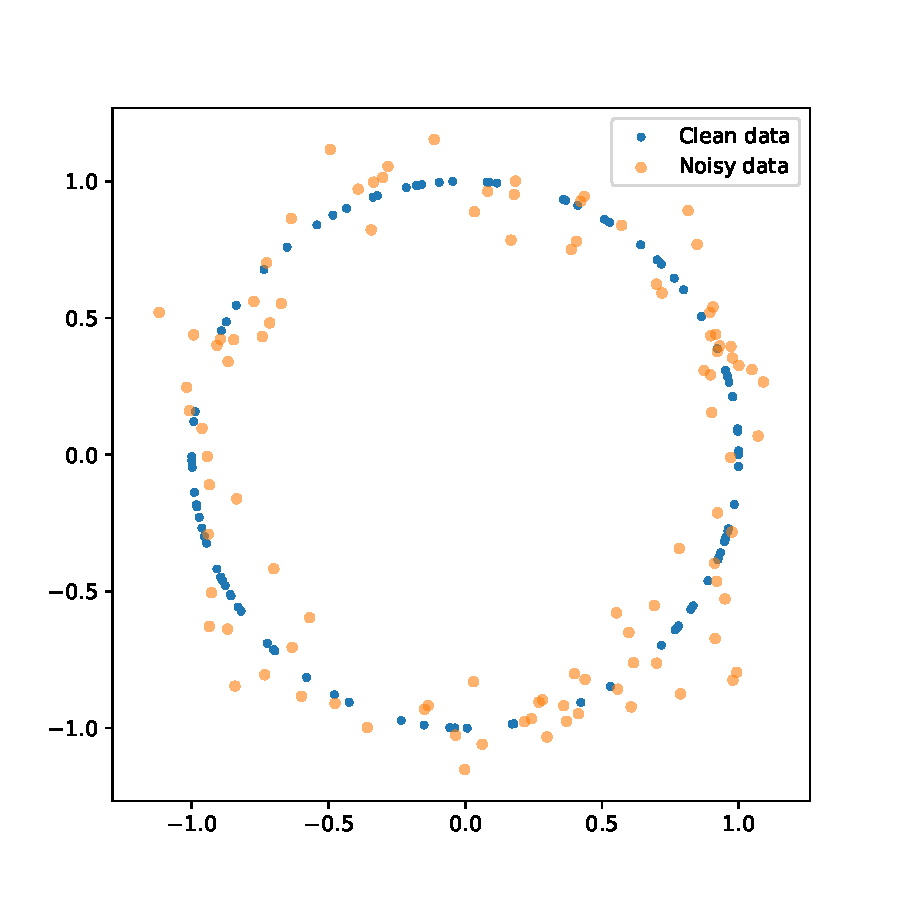
\includegraphics[width=9cm, height=8cm]{Circle_clean_noisy.pdf}
  \caption{A random sample drawn from the unit circle and one drawn from the same circle with additional Gaussian noise.}
  \label{fig:noisy_clean_circles}
\end{figure}

To compute the persistence diagrams, we will use the \textit{scikit-tda} \cite{scikittda2019} Python library. It follows the \textit{scikit} API design, making it compatible with libraries such as NumPy \cite{harris2020array}, Matplotlib \cite{Hunter:2007} or other \textit{scikit}-like libraries, for example \textit{scikit-learn} \cite{scikit-learn} (general machine learning algorithms), \textit{scikit-image} \cite{van2014scikit} (image processing algorithms) or \textit{scikit-fda} \cite{ramos-carreno++_2024_scikit-fda} (functional data analysis library). In contrast to other libraries that will be used, \textit{scikit-tda} is more high-level, trying to hide the granular details away from the user. The code for the following example can be found in the file \textit{PersistentHomology01.ipynb}.

\par
The resulting persistence diagrams can be seen on \ref{fig:clean_noisy_homologies} side by side. In both diagrams, we see a lot of blue dots at the beginning of the filtration, those being the points that quickly merge together into the single connected component -- the boundary of the circle -- and stay this way, its homology class never dying and displayed at the top of the diagram on the infinity line. The first persistent homology groups inform us about the presence of a one-dimensional hole in both diagrams, characterized by the one orange dot near the top.

In the noisy version there appear multiple smaller orange dots near the diagonal at the start; their presence signalling some sort of topological and stochastic noise since those classes die quickly after being born. It is also worthwhile to point out that the significant orange dot appears on different scales for the clean and noisy circle, marking another difference between the two that would be harder to confirm purely through some statistical testing.

\begin{figure}
    \centering
    \subfloat[\centering Clean sample]{{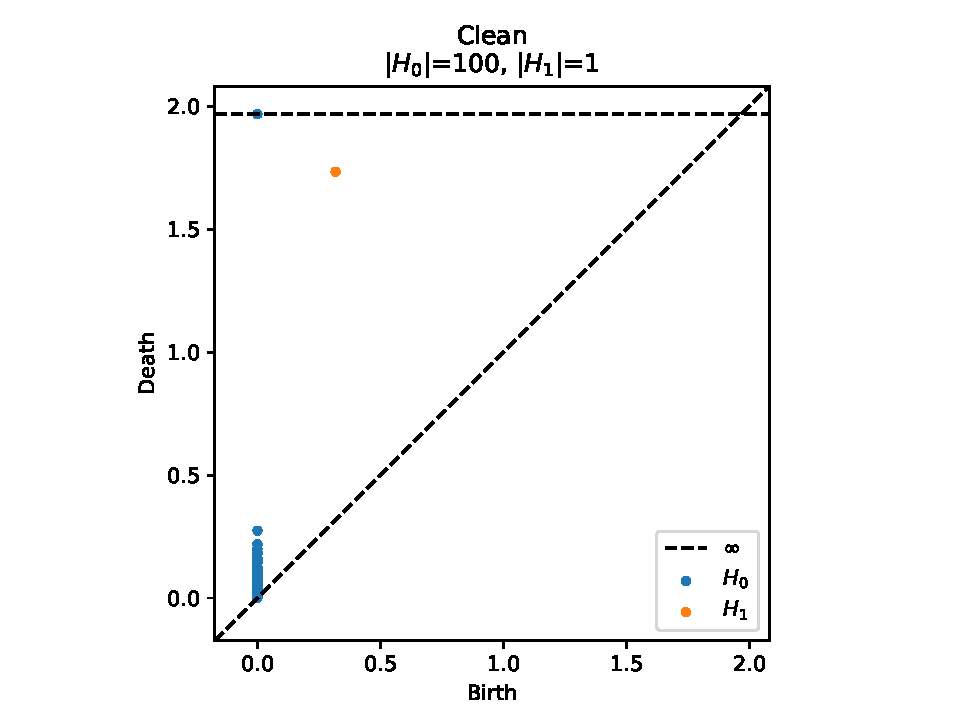
\includegraphics[width=8cm]{Clean_homology.pdf}}}
    \qquad
    \subfloat[\centering Noisy sample]{{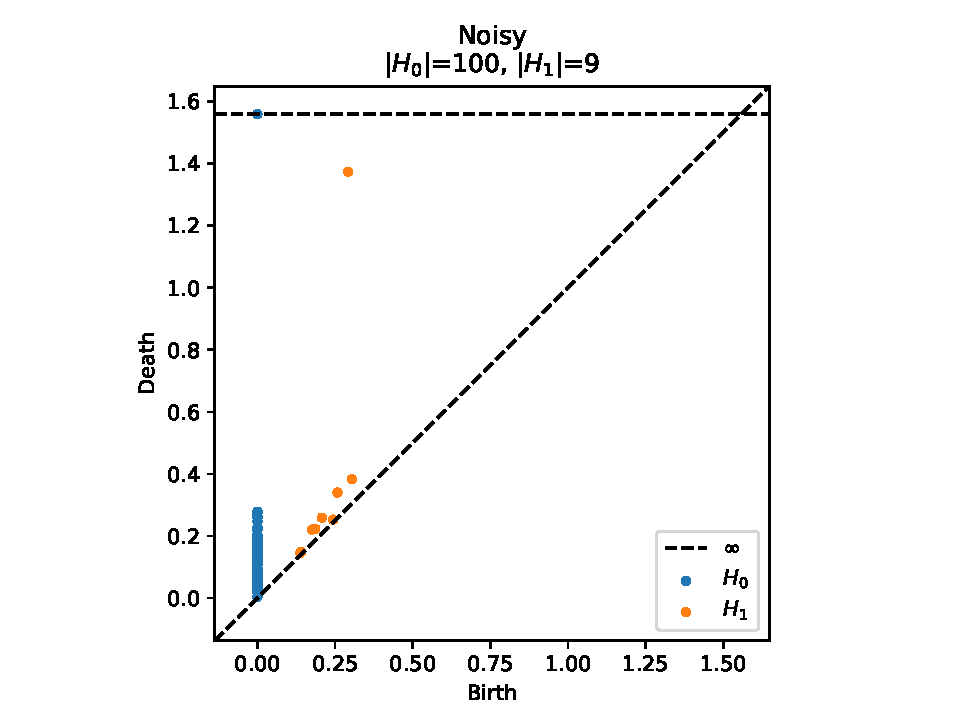
\includegraphics[width=8cm]{Noisy_homology.pdf}}}
    \caption{Persistence diagrams of the random ``clean'' and noisy circle samples. We can see that the essential features are preserved even in the presence of noise.}
    \label{fig:clean_noisy_homologies}
\end{figure}
